%%law inductive

Following is a demonstration of the discretized form from the inductive law (\ref{eq:maxwell_1}). Considering the path integral in a single element edge like Fig.  \ref{fig:FIT_max_integral1}, the left side of (\ref{eq:maxwell_1}) can be presented as  (\ref{eq:inductive_left}). 

\begin{figure}[!ht]
\centering
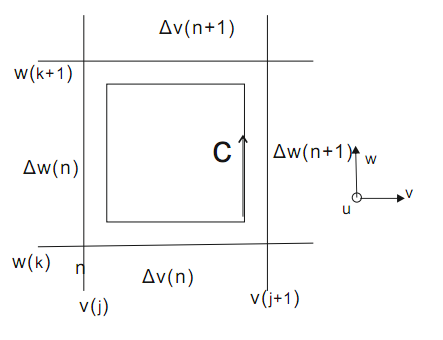
\includegraphics[width=0.45\textwidth]{bilder/FIT_max_integral1}
\caption{ Path integral along edges of one single elemental plane $A_{u}(n)$\cite{ script_FeldSim}.}
\label{fig:FIT_max_integral1}
\end{figure}

\begin{figure}[!ht]
\centering
\subfigure[Discrete electric field strength components distribute at edges of grids.]{
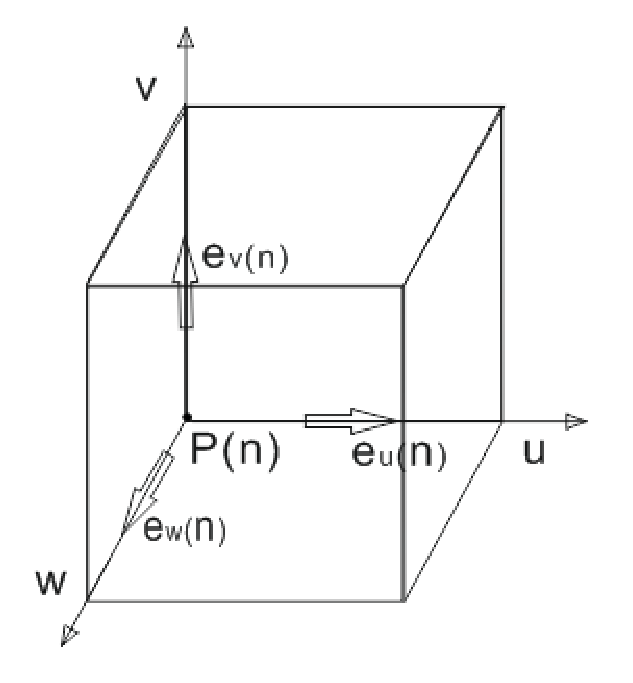
\includegraphics[width=0.4\textwidth]{bilder/FIT_max_integral2}
\label{fig:FIT_max_integral2}
}
\hfill
\subfigure[Discrete magnetic flux density components distribute at planes of grids.]{
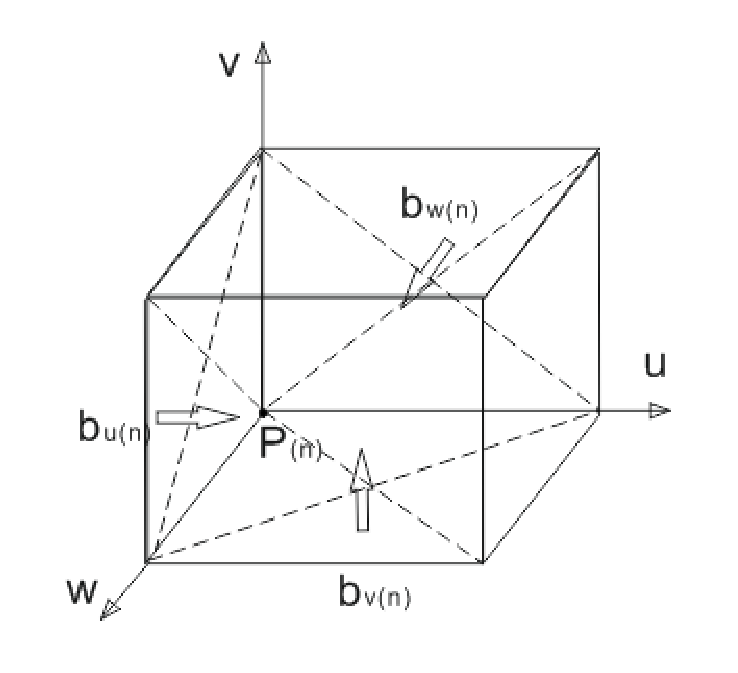
\includegraphics[width=0.5\textwidth]{bilder/FIT_max_integral3}
\label{fig:FIT_max_integral3}
}
\caption{Allocations of components at grids\cite{ script_FeldSim}.}
\end{figure}

\begin{equation}
\int_{C}\vec{E}\cdot d\vec{s}
=\underbrace{\int_{\Delta v(n)}\vec{E}\cdot d\vec{s}}_{\widehat{e}_{v}(n)}
+\underbrace{\int_{\Delta w(n+M_{v})}\vec{E}\cdot d\vec{s}}_{\widehat{e}_{w}(n+M_{v})}
-\underbrace{\int_{\Delta v(n+M_{w})}\vec{E}\cdot d\vec{s}}_{\widehat{e}_{v}(n+M_{w})}
-\underbrace{\int_{\Delta w(n)}\vec{E}\cdot d\vec{s}}_{\widehat{e}_{w}(n)}
\label{eq:inductive_left}
\end{equation}

Where $\widehat{e}(n)$ is so called  electric grid voltage and has the following relation with electric field strength $e(n)$ (seeing Fig. \ref{fig:FIT_max_integral2})
\begin{equation}
 e_{v}(n)=\frac{\widehat{e}_{v}(n)}{\Delta v(n)}
\label{eq:e_field}
\end{equation}
Meanwhile the right hand side of (\ref{eq:maxwell_1}) approximates to (\ref{eq:inductive_right})
\begin{equation}
-\iint_{A_{u}(n)}\frac{\partial\vec{B}}{\partial t}\cdot\mathrm{d}\vec{A} 
=-\iint_{A_{u}(n)}\frac{\partial B^{*}_{u}}{\partial t}\cdot\mathrm{d}A
\approx -\frac{\partial}{\partial t}b_{u}(n)A_{u}(n)
\label{eq:inductive_right}
\end{equation}
Where $A_{u}(n)=\Delta v(n)\Delta w(n)$ and $b_{u}(n)$ (Fig. \ref{fig:FIT_max_integral3}) is magnetic flux density, given by
\begin{equation}
 b_{u}(n)=\frac{\widehat{\widehat{b}}_{u}(n)}{\Delta A_{u}(n)} \text{,}
\label{eq:b_flux_density}
\end{equation}
 and magnetic grid flux $\widehat{\widehat{b}}_{u}(n)$, given by
\begin{equation}
\widehat{\widehat{b}}_{u}(n)=\iint_{A_{u}(n)}\vec{B}\cdot\mathrm{d}\vec{A} \text{.}
\label{eq:mag_fluxe}
\end{equation}
From equations (\ref{eq:inductive_left}-\ref{eq:mag_fluxe}) we obtain the difference form (\ref{eq:inductive_integral}) of the inductive equation at one single elemental plane:
\begin{equation}
\widehat{e}_{v}(n)+\widehat{e}_{w}(n+M_{v})-\widehat{e}_{v}(n+M_{w})-\widehat{e}_{w}(n)=-\frac{\partial}{\partial t}\widehat{\widehat{b}}_{u}(n)
\label{eq:inductive_integral}
\end{equation}
i.e.,
\begin{align}
\Delta v(n)e_{v}(n)&+\Delta w(n+M_{v})e_{w}(n+M_{v})\nonumber\\
-\Delta v(n+M_{w})e_{v}(n+M_{w})&-\Delta w(n)e_{w}(n)=-A_{u}(n)\frac{\partial}{\partial{t}}b_{u}(n) 
\label{eq:inductive_sample}
\end{align}
By merging electric field-strength $e(n)$ and magnetic flux density $b(n)$ of all grids into vectors we obtain
\begin{equation*}
e_{u}:=
\begin{pmatrix}
e_{u}(1)&\\
\vdots&\\
e_{u}(N_{p})&
\end{pmatrix},
e_{v}:=
\begin{pmatrix}
e_{v}(1)&\\
\vdots&\\
e_{v}(N_{p})&
\end{pmatrix},
e_{w}:=
\begin{pmatrix}
e_{w}(1)&\\
\vdots&\\
e_{w}(N_{p})&
\end{pmatrix},
e:=
\begin{pmatrix}
e_{u}&\\
e_{v}&\\
e_{w}&
\end{pmatrix},
\label{eq:vector_e_field}
\end{equation*}
\begin{equation*}
b_{u}:=
\begin{pmatrix}
b_{u}(1)&\\
\vdots&\\
b_{u}(N_{p})&
\end{pmatrix},
b_{v}:=
\begin{pmatrix}
b_{v}(1)&\\
\vdots&\\
b_{v}(N_{p})&
\end{pmatrix},
b_{w}:=
\begin{pmatrix}
b_{w}(1)&\\
\vdots&\\
b_{w}(N_{p})&
\end{pmatrix},
b:=
\begin{pmatrix}
b_{u}&\\
b_{v}&\\
b_{w}&
\end{pmatrix}.
\label{eq:vector_m_flux_density}
\end{equation*}
Expanding the relation (\ref{eq:inductive_sample}) to all grid cells \cite{FIT_discrete_method,FIT_discrete_electrommagnetism} we arrive at the discrete form of inductive equation:
\begin{equation}
CD_{s}e=-D_{A}\frac{\partial}{\partial{t}}b
\label{eq:inductive_sample_all}
\end{equation}
Where $D_{s}$ is elemental edge matrix, given by
\begin{align*}
D_{s}=
%	\begin{pmatrix}
%	\Delta u(1)&&&&&&&&\\
%	&\ddots &&&&&&&\\
%	&&\Delta u(N_{p})&&&&&&\\
%	&&&\Delta v(1)&&&&&\\
%	&&&&\ddots &&&&\\
%	&&&&&\Delta v(N_{p})&&&\\
%	&&&&&&\Delta w(1)&&\\
%	&&&&&&&\ddots &\\
%	&&&&&&&&\Delta w(N_{p})
%	\end{pmatrix}
Diag\{&\Delta u(1),\cdots,\Delta u(N_{p}),\nonumber\\
			&\Delta v(1),\cdots,\Delta v(N_{p}),\nonumber\\
			&\Delta w(1),\cdots,\Delta w(N_{p})
\} \text{.}
	%\label{eq:Ds_matrix}
\end{align*}
$D_{A}$ is elemental plane matrix, given by
\begin{align*}
D_{A}=
%	\begin{pmatrix}
%	\Delta A_{u}(1)&&&&&&&&\\
%	&\ddots &&&&&&&\\
%	&&\Delta A_{u}(N_{p})&&&&&&\\
%	&&&\Delta A_{v}(1)&&&&&\\
%	&&&&\ddots &&&&\\
%	&&&&&\Delta A_{v}(N_{p})&&&\\
%	&&&&&&\Delta A_{w}(1)&&\\
%	&&&&&&&\ddots &\\
%	&&&&&&&&\Delta A_{w}(N_{p})
%	\end{pmatrix}
Diag\{&\Delta A_{u}(1),\cdots,\Delta A_{u}(N_{p}),\nonumber\\
			&\Delta A_{v}(1),\cdots,\Delta A_{v}(N_{p}),\nonumber\\
			&\Delta A_{w}(1),\cdots,\Delta A_{w}(N_{p})
\} \text{.}
	%\label{eq:Da_matrix}
\end{align*}
$C$ is \textbf{curl} operator, given by
\begin{equation*}
C=
	\begin{pmatrix}
	0&-P_{w}&P_{v}\\
	P_{w}&0&-P_{u}\\
	-P_{v}&P_{u}&0
	\end{pmatrix} \text{.}
%\label{eq:C_matrix}
\end{equation*}
\begin{figure}[!ht]
\centering
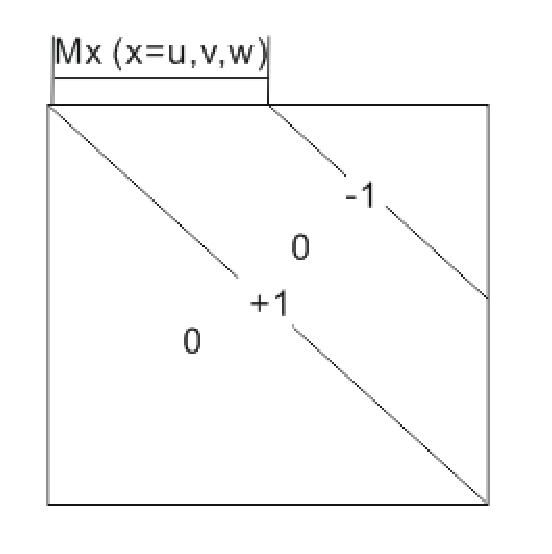
\includegraphics[width=0.35\textwidth]{bilder/P_matrix}
\caption{Structure of matrix $P_{x},(x=u,v,w)$.}
\label{fig:Matrix Px}
\end{figure}
Submatrices $P_{u},P_{v},P_{w}$ are composed of $1,-1,0$ like Fig. \ref{fig:Matrix Px}.\\
 
Alternative form of the equation (\ref{eq:inductive_sample_all}) is given in (\ref{eq:inductive_integral_all})
\begin{equation}
C\widehat{e}=-\frac{\partial}{\partial{t}}\widehat{\widehat{b}}
\label{eq:inductive_integral_all}
\end{equation}
%\widehat{e}
Where $\widehat{e}$ is electric voltage and $\widehat{\widehat{b}}$ magnetic flux.
%divergence equation
Analogy the divergence equation (\ref{eq:maxwell_4}) can also be discretized in grid $G$ and its difference form is given by 
\begin{equation*}
SD_{A}b=0
\label{eq:divergence_sample}
\end{equation*}
or
\begin{equation*}
S\widehat{\widehat{b}}=0
\label{eq:divergence_integral}
\end{equation*}
$S\in \mathbb{R}^{N_{p}\times 3N_{p}}$ represent the discrete divergence matrix, which depends on the grid topology just as the discrete $curl-Matrix$ $C$.
%S
\begin{equation*}
S=(P_{u}|P_{v}|P_{w})
\label{eq:S_matrix}
\end{equation*}
%Amp\'ere's law
For discretizing Amp\'ere's law (\ref{eq:maxwell_2}) \textbf{Dual Grid} is defined, seeing Fig. \ref{fig:dual_grid}. 

\begin{figure}[!ht]
\centering
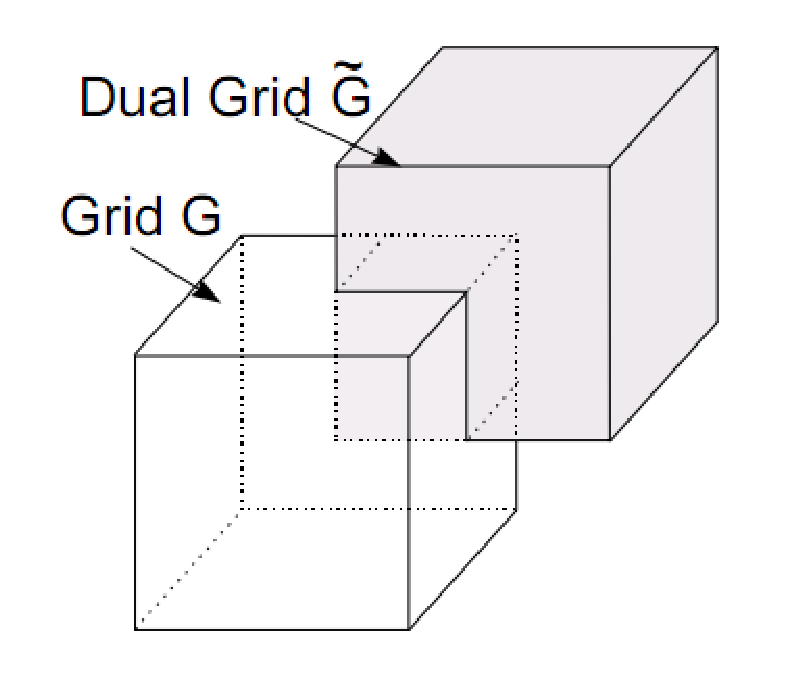
\includegraphics[width=0.5\textwidth]{bilder/dual_grid}
\caption{The allocation of the Primary Grid $G$ and Dual Grid $\tilde{G}$\cite{FIT_discrete_electrommagnetism}.}
\label{fig:dual_grid}
\end{figure}
Then the discretized form of (\ref{eq:maxwell_2}) in dual grid is obtained like
\begin{equation*}
\tilde{C}\tilde{D}_{s}D_{\mu^{-1}}b=\tilde{D}_{A}(D_{\epsilon}\frac{\mathrm{d}}{\mathrm{dt}}e+D_{\kappa}e+j)
\label{eq:ampere}
\end{equation*}
or
\begin{equation*}
\tilde{C}\widehat{h}=\frac{\mathrm{d}}{\mathrm{dt}}\widehat{\widehat{d}}+\widehat{\widehat{j}}_{L}+\widehat{\widehat{j}}_{S}
\label{eq:ampere_sample}
\end{equation*}

Where $\bar{\epsilon}$ is average dielectric constant. $ D_{\epsilon}$ is the average dielectric matrix. $\tilde{C}$ represents the $curl-operator$ in dual grid.
With the help of dual grid cells Gauss' law (\ref{eq:maxwell_3}) in integral form can be discretized\cite{script_FeldSim} as following:
\begin{equation*}
\tilde{S}\widehat{\widehat{d}}=q
\label{eq:gausslaw}
\end{equation*}
or
\begin{equation*}
\tilde{S}\tilde{D}_{A}D_{\epsilon}e=\tilde{D}_{V}\rho_{D}
\label{eq:gausslaw_sample}
\end{equation*}
Where $\rho_{D}$ is the vector of the charge density in grid cells.

\begin{equation*}
\tilde{S}=(\tilde{P}_{u}|\tilde{P}_{v}|\tilde{P}_{w})=(-P_{u}^{T}|-P_{v}^{T}|\-P_{w}^{T})
\label{eq:dual_S_matrix}
\end{equation*}
